%----------------------------------- Math notes ----------------------------


%--------------------------------
% Latex document setup:
%--------------------------------
%\documentclass{article}
\documentclass{book}
\usepackage{graphicx}		% Required for the inclusion of images
\usepackage{amsmath} 		% Required for some math elements 
\usepackage{amssymb}
\usepackage{listings}
\usepackage{enumerate}
\usepackage[font=small,labelfont=bf,width=0.8\linewidth]{caption}
\usepackage{cite}
\usepackage{tabularx}
%\usepackage{times} 		% Uncomment to use Times New Roman 



%--------------------------------
% Package for hyperlinking to any 
% word in document:
%--------------------------------
%\usepackage[colorlinks]{hyperref}      % Two different setup syntaxes
\usepackage{hyperref}                   
\hypersetup{
    colorlinks = true,
    linkcolor=cyan,
}



%--------------------------------
% Paragraph spacing:
%--------------------------------
\setlength{\parskip}{0.4em}    



%--------------------------------
% Set bullet symbols: (for 
% itemize)
%--------------------------------
\renewcommand{\labelitemi}{$\circ$}
\renewcommand{\labelitemii}{$\circ$}
\renewcommand{\labelitemiii}{$\circ$}
\renewcommand{\labelitemiv}{$\circ$}

%----------------------------------------------
% Custom commands:
%----------------------------------------------
% keywords : tools, macros, commands

% macro test
\def\hore{$\alpha\delta\epsilon$}       % works without math mode
\def\horeto{\alpha\delta\epsilon}       % works in math mode


% Define a macro for placing vline between cells in table: 
% \def\individualvline{\hfil\kern\arraycolsep\vline\kern-\arraycolsep\hfilneg}



%----------------------------------------------
% Title page:
%----------------------------------------------
\title{Analysis of Titanic data} 
\author{Samuel Knudsen} % Author name
%\date{Starting December 18, 2020, Graz} 
\date{Last update: \today}


%----------------------------------------------
% Documents starts here:
%----------------------------------------------
\begin{document}
\maketitle



\begin{figure}
    \centering
    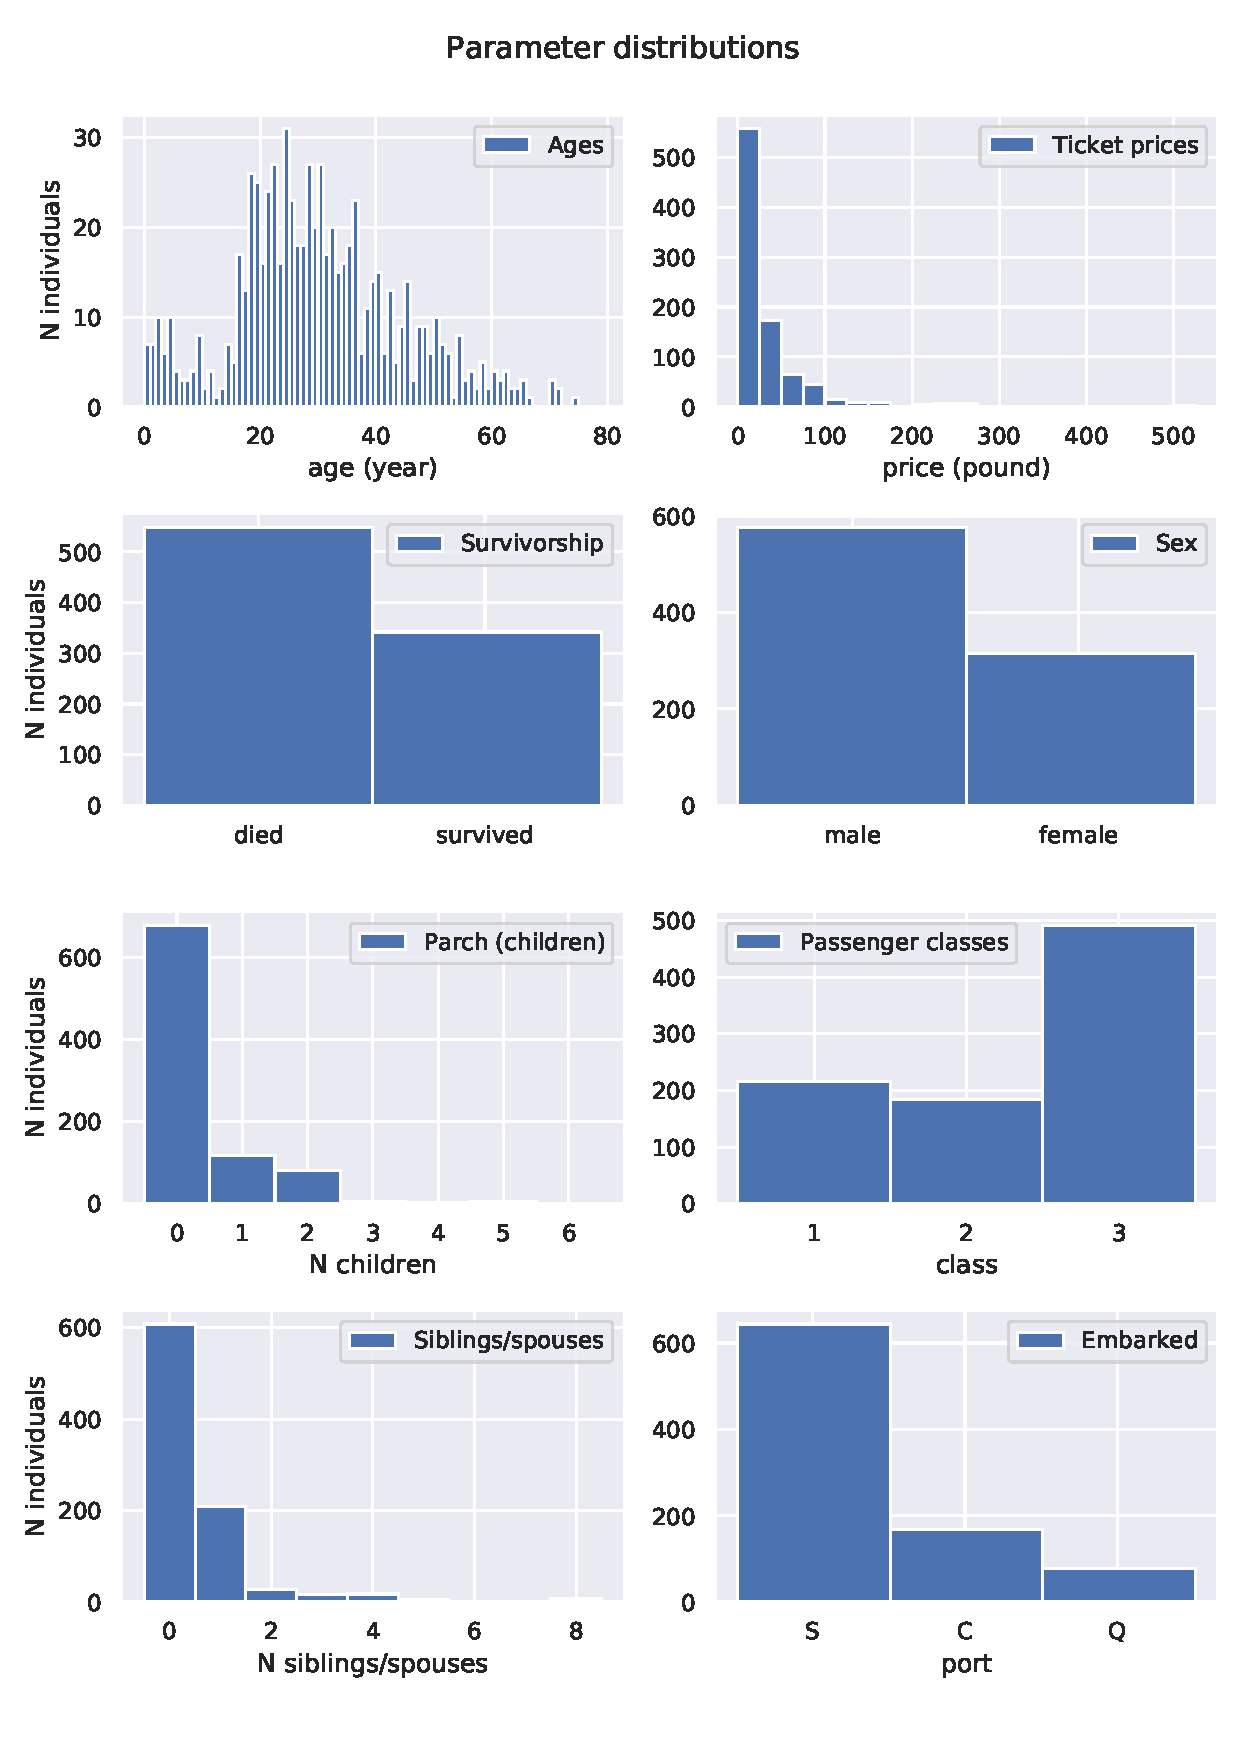
\includegraphics[scale=0.67]{../figs/distributions.pdf}%
\end{figure}


\clearpage
\begin{figure}
    \centering
    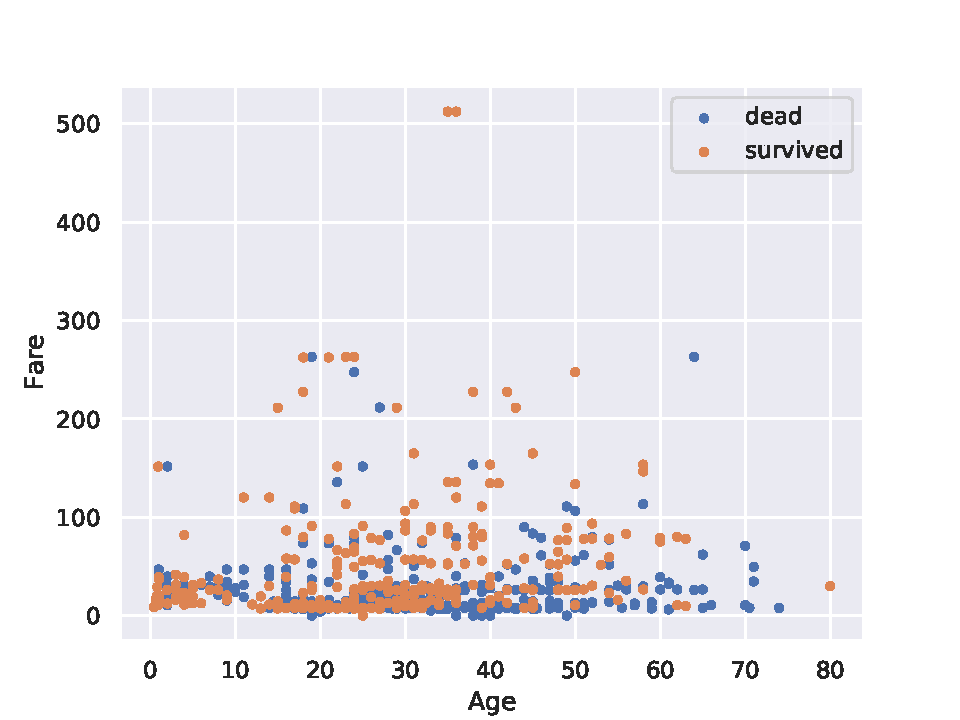
\includegraphics[scale=.75]{../figs/scatter2d_Age_Fare.pdf}
    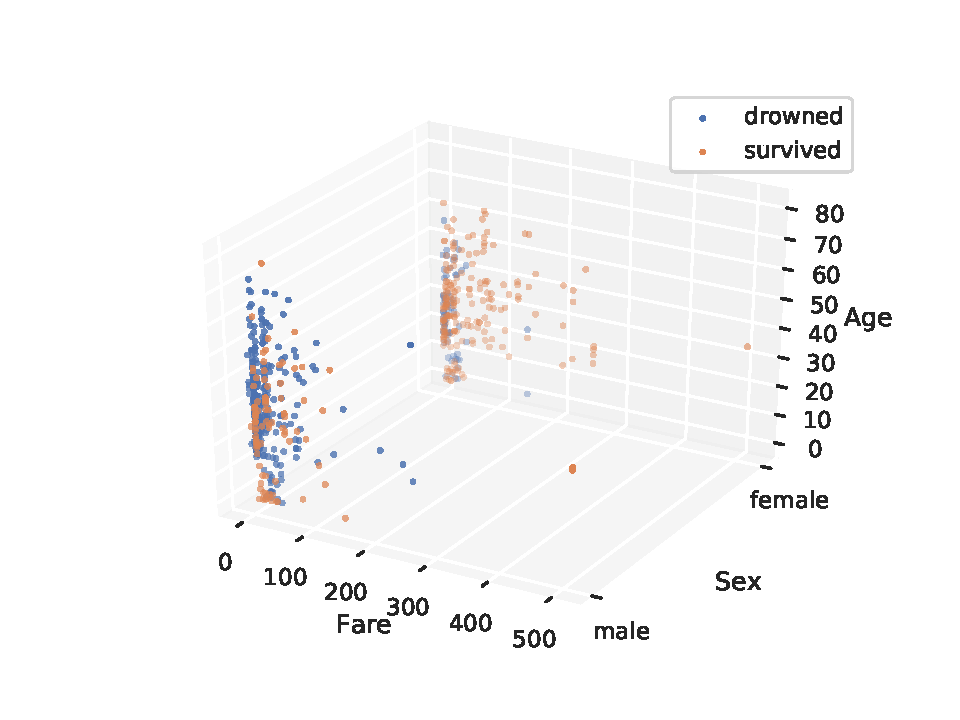
\includegraphics[scale=0.7]{../figs/scatter3d.pdf}%
\end{figure}

% \begin{figure}[h]
%     \centering
%     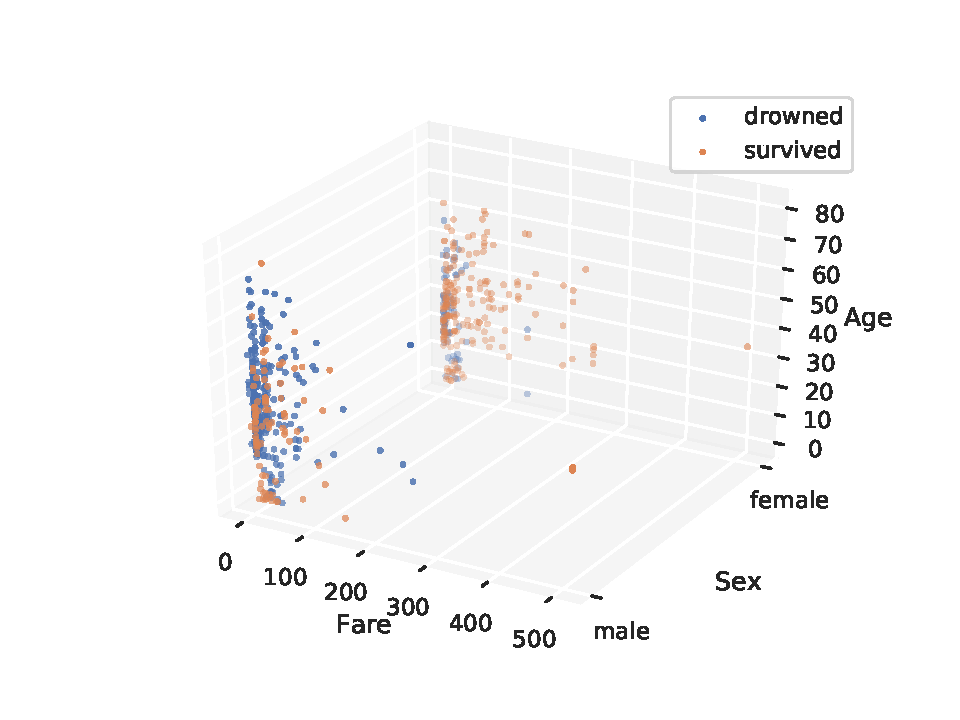
\includegraphics[scale=0.7]{../figs/scatter3d.pdf}%
% \end{figure}


\clearpage
\begin{equation}
    %p(\text{survival}, \text{sex}) = p(\text{survival} | \text{sex})p(\text{sex})
    \begin{split}
        p(A,B) & = p(A| B)p(B) \\
        p(B,A) & = p(B|A)p(A)
    \end{split}
\end{equation}

and
\begin{equation}
    p(A,B) = p(B,A)
\end{equation}
meaning 
\begin{equation}
    p(A|B) =  \frac{p(B|A)p(A)}{p(B)}
\end{equation}


% Bayesian analysis

\begin{equation}
    p(\text{survival} | \text{gender}) = \frac{p( \text{gender}|\text{survival} )p(\text{survival})}{p(\text{gender})}
\end{equation}

\clearpage
\section{Training a neural network to predict survival}
\begin{figure}[h]
    \centering
    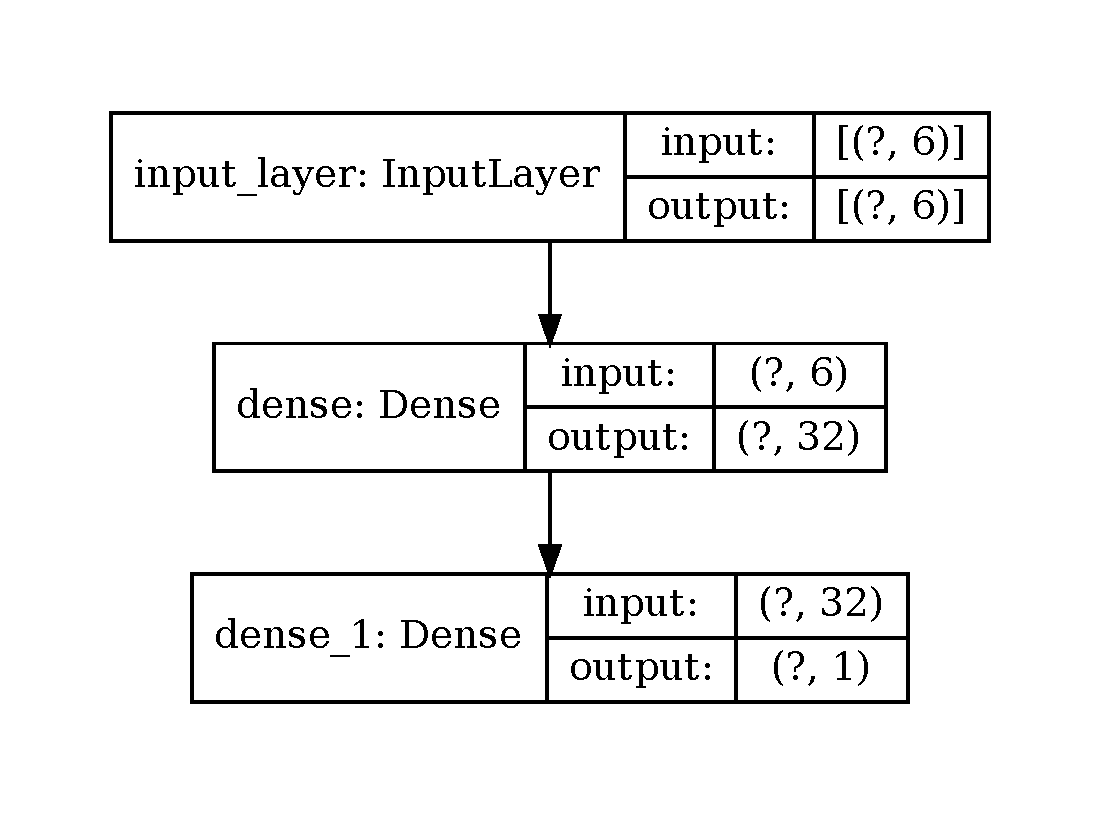
\includegraphics[scale=.4]{../figs/model.pdf}
    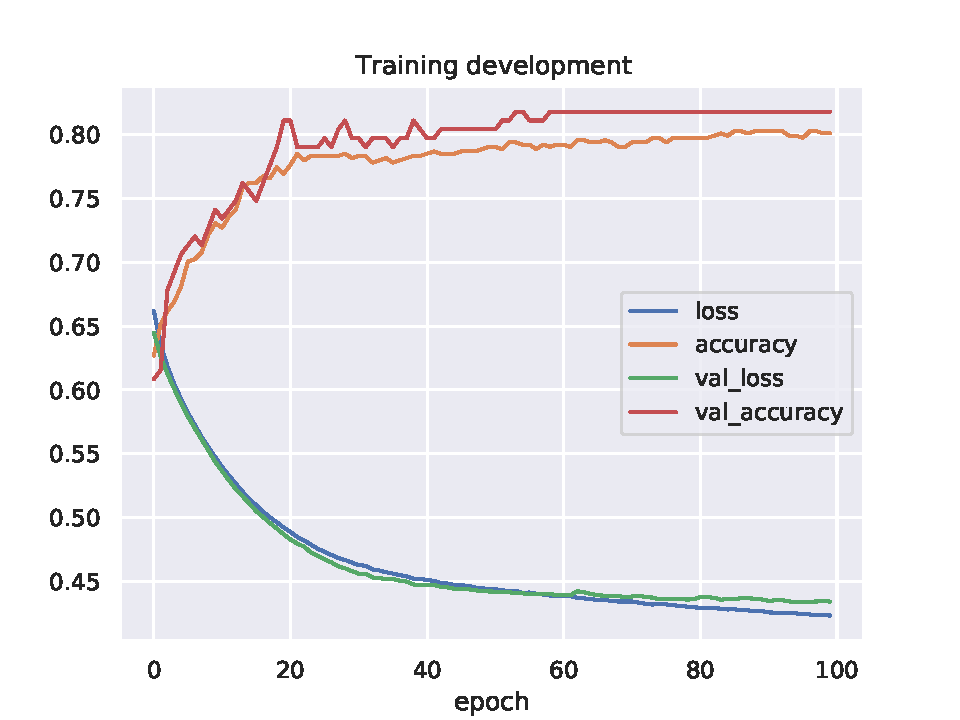
\includegraphics[scale=.65]{../figs/training_development.pdf}
\end{figure}
% \begin{figure}[h]
%     \centering
%     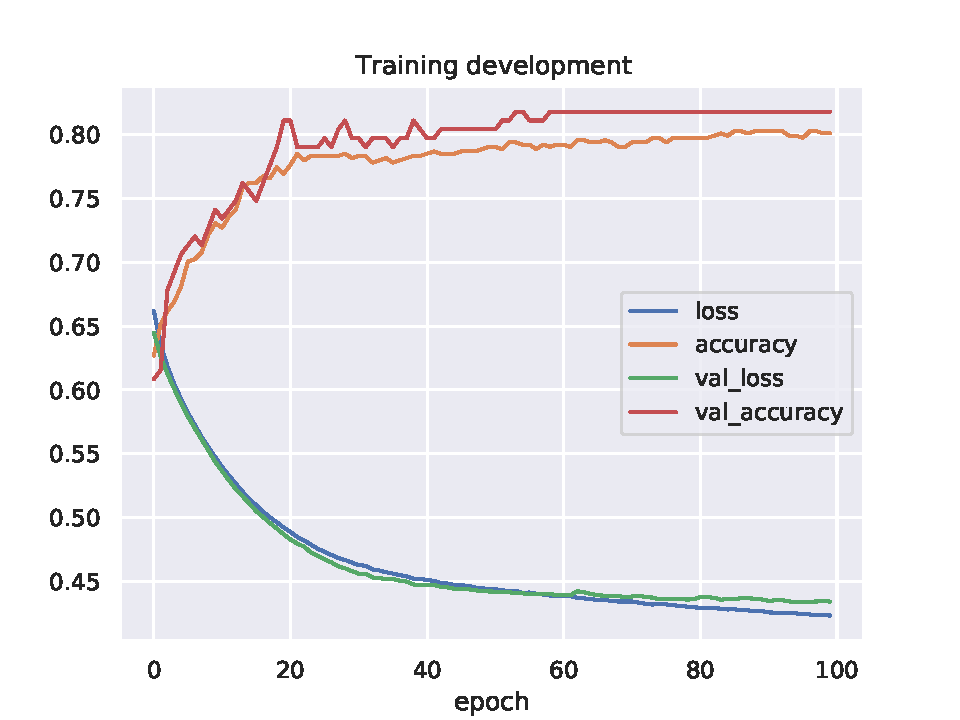
\includegraphics[scale=.65]{../figs/training_development.pdf}%
% \end{figure}

% \clearpage
% \begin{figure}
% 	\centering
% 	\includegraphics[scale=0.65]{../figs/fare_histogram.pdf}
% \end{figure}


% \begin{figure}
% 	\centering
% 	\includegraphics[scale=0.65]{../figs/survival_histogram.pdf}
% \end{figure}








%%---------------------------------------
%% Tabular of some sort:
%%---------------------------------------
%\begin{center}
%\begin{tabular}{l r}
%A &  B \\ 
%C & D
%\end{tabular}
%\end{center}



%---------------------------------------
% Table: 
%---------------------------------------
% \begin{table}
% 	\centering
% 	\begin{tabular}{ l | l | r  }
% 	 Population & Parameter & Value \\
% 	 \hline
% 	 Excitatory  & 	 & \\
% 	\end{tabular}

% 	\caption{}

% 	\label{lsm_table}
% \end{table}




%---------------------------------------
% Itemize
%---------------------------------------

% \begin{itemize}
% 	\item Something

% 	\begin{enumerate}
% 		\item Something else

%     	\end{enumerate}
% \end{itemize}
%
%
%---------------------------------------
%% Figure
%---------------------------------------
%
%\begin{figure}
%	\centering
%	\includegraphics[scale=0.6]{some_fig.jpg}
%	\caption{some caption}
%	\label{some_label}
%\end{figure}
%
%
%---------------------------------------
% BIBLIOGRAPHY
%---------------------------------------

%%\clearpage
%%\bibliography{citations.bib}
%
%\bibliographystyle{apalike}
%\bibliographystyle{ieeetr}
%\bibliography{sample}




\end{document}

